%% chapter 4

\chapter{实验数据分析}

\section{测序数据预处理}
  通过图\ref{fig:expr-fig1}a所示的流程,我们获取了小鼠垂体细胞的单细胞测序数据。将测序得到的fastq文件利用CellRanger进行上游分析,序列回帖参考基因组选用Ensembl(GRCm38)。回帖得到的基因表达矩阵通过Scater\cite{mccarthy2017scater}进行质量控制,筛除低质量细胞,再用Seurat v3\cite{butler2018integrating,stuart2019comprehensive}进行基础下游分析。

\begin{figure}[!htb]
  \centering
  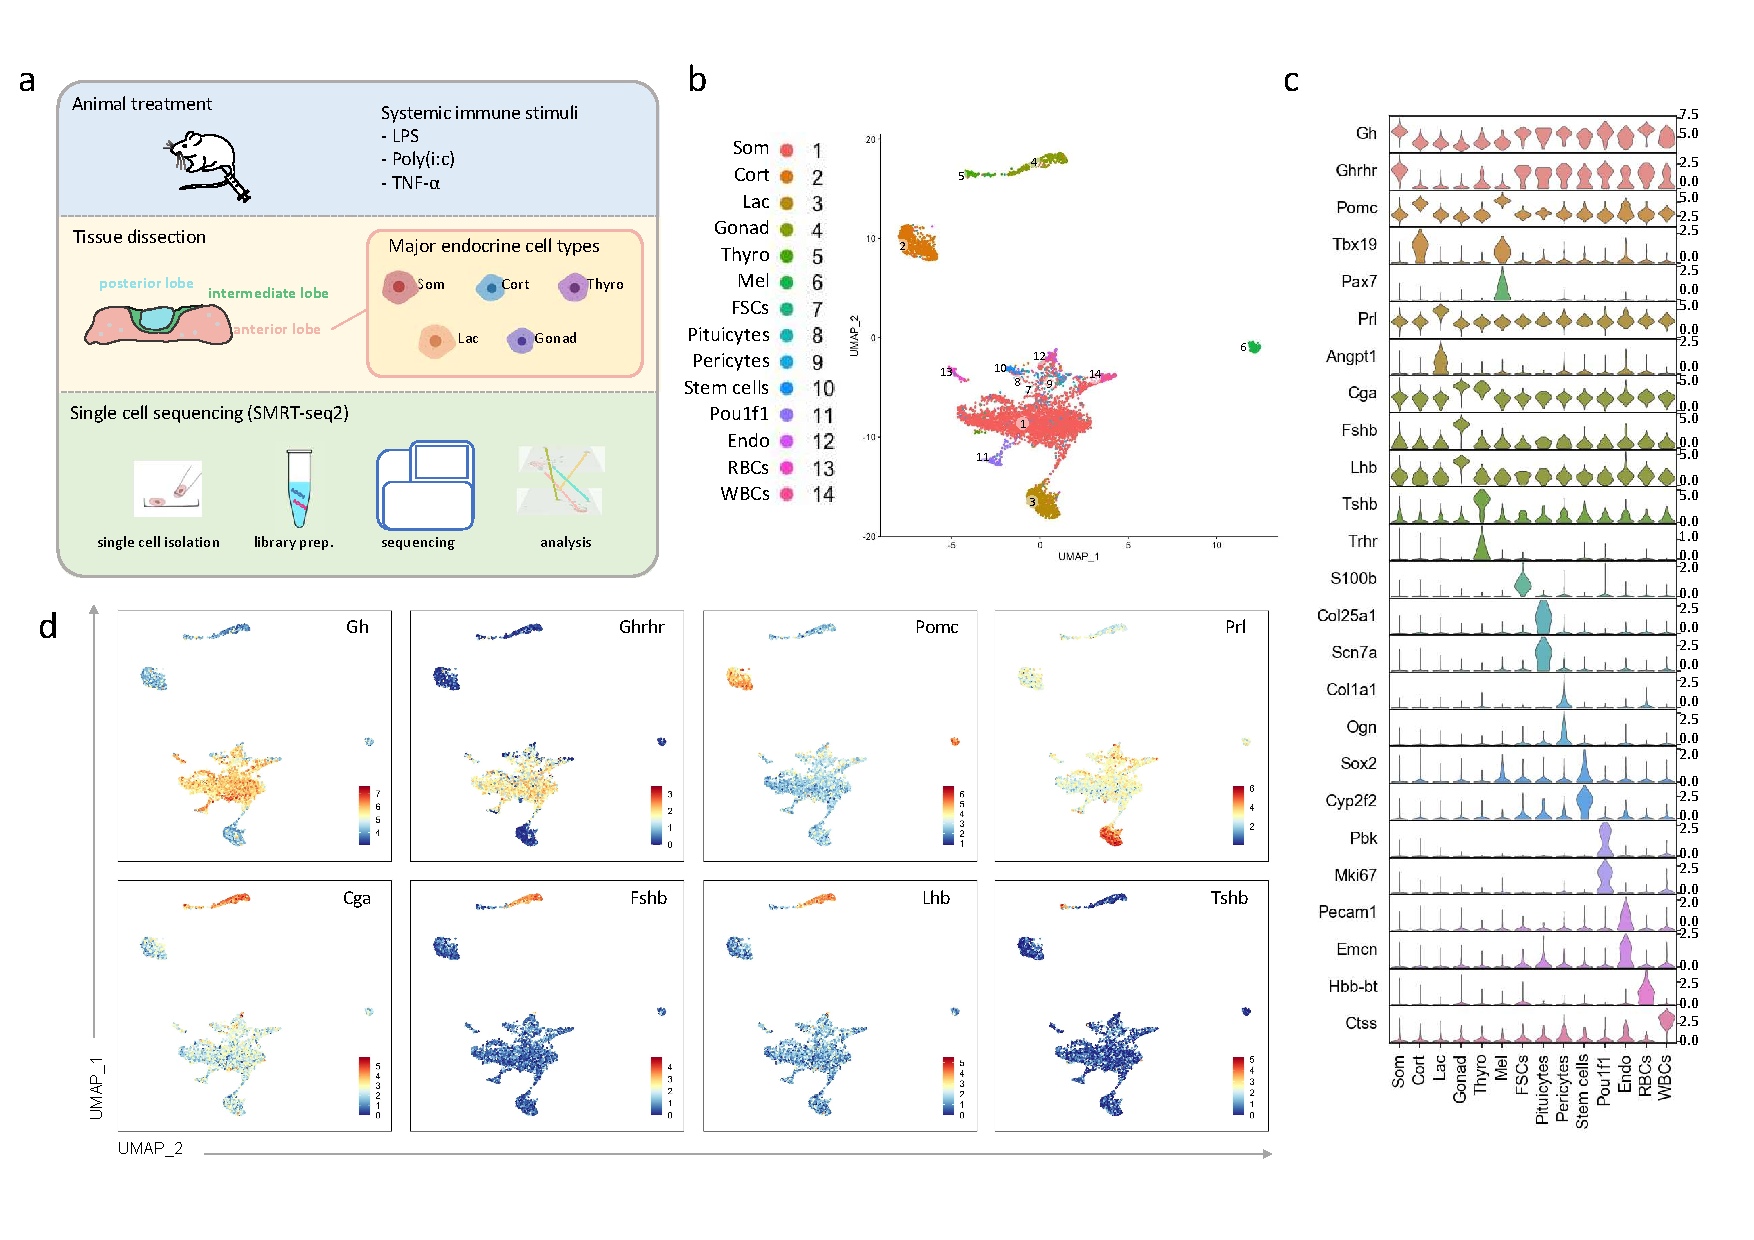
\includegraphics[width=1.0\textwidth]{figs/expr-fig1.pdf}
  \caption{单细胞测序数据预处理}
  \label{fig:expr-fig1}
\end{figure}

\subsection{Scater质控}
  将测序数据读入R工作环境中,将表达矩阵转换为SingleCellExperiment(SCE)对象,对该SCE对象依次在细胞水平(Cell-level QC)、基因水平(Feature-level QC)以及变量水平(Variable-level QC)执行质控。在细胞水平质控中,去除文库含量小(low library size)、基因含量少(low features)和线粒体基因含量高(high mitochondrial percentage)的细胞;在基因水平质控中,去除表达量为0的基因以及线粒体基因、核糖体基因,以避免在PCA部分影响主成分判别;在变量水平中,对每个变量方差解释的贡献率(variance explained)做统计,查看是否有异常变量出现。

  通过STAR-featureCounts上游管线处理后,我们共收集到6727个细胞,平均每个细胞检测到3546个基因。在经过Scater质控后,保留了5506个细胞。
\subsection{Seurat初步分析}
  经过质控处理后的数据转换为Seurat对象,执行Seurat基础分析流程:归一化、特征选择、放缩、线性降维、构建最短临近图、Leiden聚类以及UMAP可视化。

  在此基础上,结合聚类信息以及中枢神经系统各细胞类型已知的基因marker(表\ref{tab:gene-marker}),对数据进行细胞类型注释。我们在垂体腺中鉴定了6个主要细胞簇(Somatotropes,Corticotropes,Melanotropes,Lactotropes,Thyrotropes,Gonadotropes),这与先前的知识是一致的。详见图\ref{fig:expr-fig1}。
\begin{table}[ht]
    \centering
    \caption{中枢神经系统各细胞类型已知的基因marker}
    \label{tab:gene-marker}
    \begin{tabular}{ll}
        \toprule
        细胞类型 & 基因marker \\
        \midrule
        Somatotropes & Gh, Ghrhr, Pappa2, Gnmt \\
        Lactotropes & Prl, Angpt1 \\
        Corticotropes & Pomc, Crhr1, Tbx19 \\
        Melanotropes & Pomc, Tbx19, Pax7, Pcsk2, Rbfox3 \\
        Gonadotropes & Fshb, Lhb, Gnrhr, Cga, Nr5a1 \\
        Thyrotropes & Tshb, Trhr, Cga \\
        Pou1f1 progenitors & Pbk, Top2a, Mki67 \\
        RBCs & Hbb-bt, Hbb-bs \\
        WBCs & C1qa, Ctss, Ptprc \\
        Folliculostellate cells & S100b, Fxyd1 \\
        Endothelial cells & Pecam1, Emcn, Plvap \\
        Pituicytes & Gja1, Scn7a, Col25a1 \\
        Pericytes & Colia1, Dcn, Ogn, Lum, Pdgfrb \\
        Stem cells & Sox2, Aldh3a1, Aldh1a2, Cgp2f2 \\
        \bottomrule
    \end{tabular}
\end{table}

  在这项研究中,我们主要关注的是系统性神经炎症对于垂体细胞的单细胞转录水平影响。因而,我们依据上面得到的细胞注释对数据进行筛选,只留下Somatotropes、Corticotropes、Lactotropes、Thyrotropes以及Gonadotropes五类细胞,共3788个细胞。我们之后的分析便都在此数据上开展。

\section{测序数据SCENIC分析}
  我们对筛选出来的测序数据进行SCENIC分析,以推断其潜在转录因子及对应目的基因。这一步的输出是一个AUC-score矩阵,矩阵的每一个单元表示每一个细胞中对每个基因集合的整体趋势评分,当其符号为正时上调,反之下调。我们对该矩阵进行降维聚类,并用其聚类结果作为细胞是否处于炎症状态的判别标准,其原因已在相关工作的基因调控网络部分说明。使用该聚类结果标注的基因表达矩阵降维结果展示在图\ref{fig:expr-fig2}a,b。对于每一类细胞,该分类结果可以很好地匹配UMAP可视化后的数据分布。

\begin{figure}[!htb]
  \centering
  \includegraphics[width=1.0\textwidth]{figs/expr-fig2.pdf}
  \caption{单细胞测序数据SCENIC分析}
  \label{fig:expr-fig2}
\end{figure}

\subsection{分析处理条件与垂体细胞状态之间的关系}
  在我们所构建小鼠炎症模型中,我们依据免疫刺激剂、给药剂量与恢复时间尺度等因素建立了一系列实验。为了揭示这一系列因素与垂体细胞状态之间的关系,我们将这些处理条件与SCENIC聚类结果进行整合,如图\ref{fig:expr-fig2}c所示。

  我们可以看到所有注射saline的处理组,基本都处于健康(healthy)状态。除此之外,还有注射LPS的处理组也对应到了健康(healthy)状态。通过观察给药剂量与恢复时间尺度因素,我们可以发现这些细胞大多是注射低剂量LPS或者经历了长时程的恢复,在这种情况下神经系统仅有少量垂体细胞处于免疫应激状态。相比之下,注射高剂量LPS且仅经历短时程恢复的处理组则大多处于炎症(inflammation)状态。

\subsection{分析不同细胞在炎症状态下的基因表达差异}
  我们进一步比较了垂体中不同细胞在炎症状态下的基因表达差异,见图\ref{fig:expr-fig2}d。该图的上半部分是垂体各类细胞在其对应基因marker上的基因表达热图。同类细胞对应的基因marker无论中枢神经系统是否处于炎症状态,都会在该类细胞中稳定表达。然后,我们对每一类细胞分析其炎症状态与健康状态下的差异表达基因集合,并将其整合,便得到了该图的下半部分。

  我们发现同处于炎症状态,垂体中不同细胞应对炎症所做出的基因表达调整并不一致。例如,在炎症状态Somatotropes中上调最显著的基因集合并不是在炎症状态Corticotropes中上调最显著的基因集合。这便说明,在中枢神经内分泌系统处于炎症状态时,垂体内各类细胞会采取不同的应激方式,组成一个调节炎症反应的复杂系统。

\subsection{分析导致炎症状态的转录因子}
  我们依据SCENIC过程得到的AUC-score矩阵,统计出每个转录因子的AUC-score密度分布,我们希望找到具备双峰分布或者重尾分布的转录因子。对这些转录因子的分布进行自适应二值化,我们发现其标签可以和之前使用SCENIC聚类结果判定的细胞状态很好地匹配起来(见图\ref{fig:expr-fig3})。

  我们通过上面过程找到的转录因子涉及Stat、Irf以及Nfkb等转录因子家族,这些转录因子大多是与免疫过程相关的。例如,Irf7编码干扰素调节因子7,以往实验数据表明其在病毒诱导的细胞基因(包括I型干扰素基因)的转录中起作用。这些转录因子并没有像之前分析的差异表达基因那样展现出细胞种类特异性,而是在整个炎症状态的垂体细胞中广泛表达。

  这就表明Stat、Irf以及Nfkb等转录因子家族在垂体参与中枢神经内分泌炎症调节过程中扮演着重要的角色,影响着各类垂体细胞的调控路径。换句话说,Stat、Irf以及Nfkb等转录因子家族是垂体参与中枢神经内分泌炎症调节过程中的Master Regulator Genes(MRs)\cite{mattick2010global}。

\begin{figure}[!htb]
  \centering
  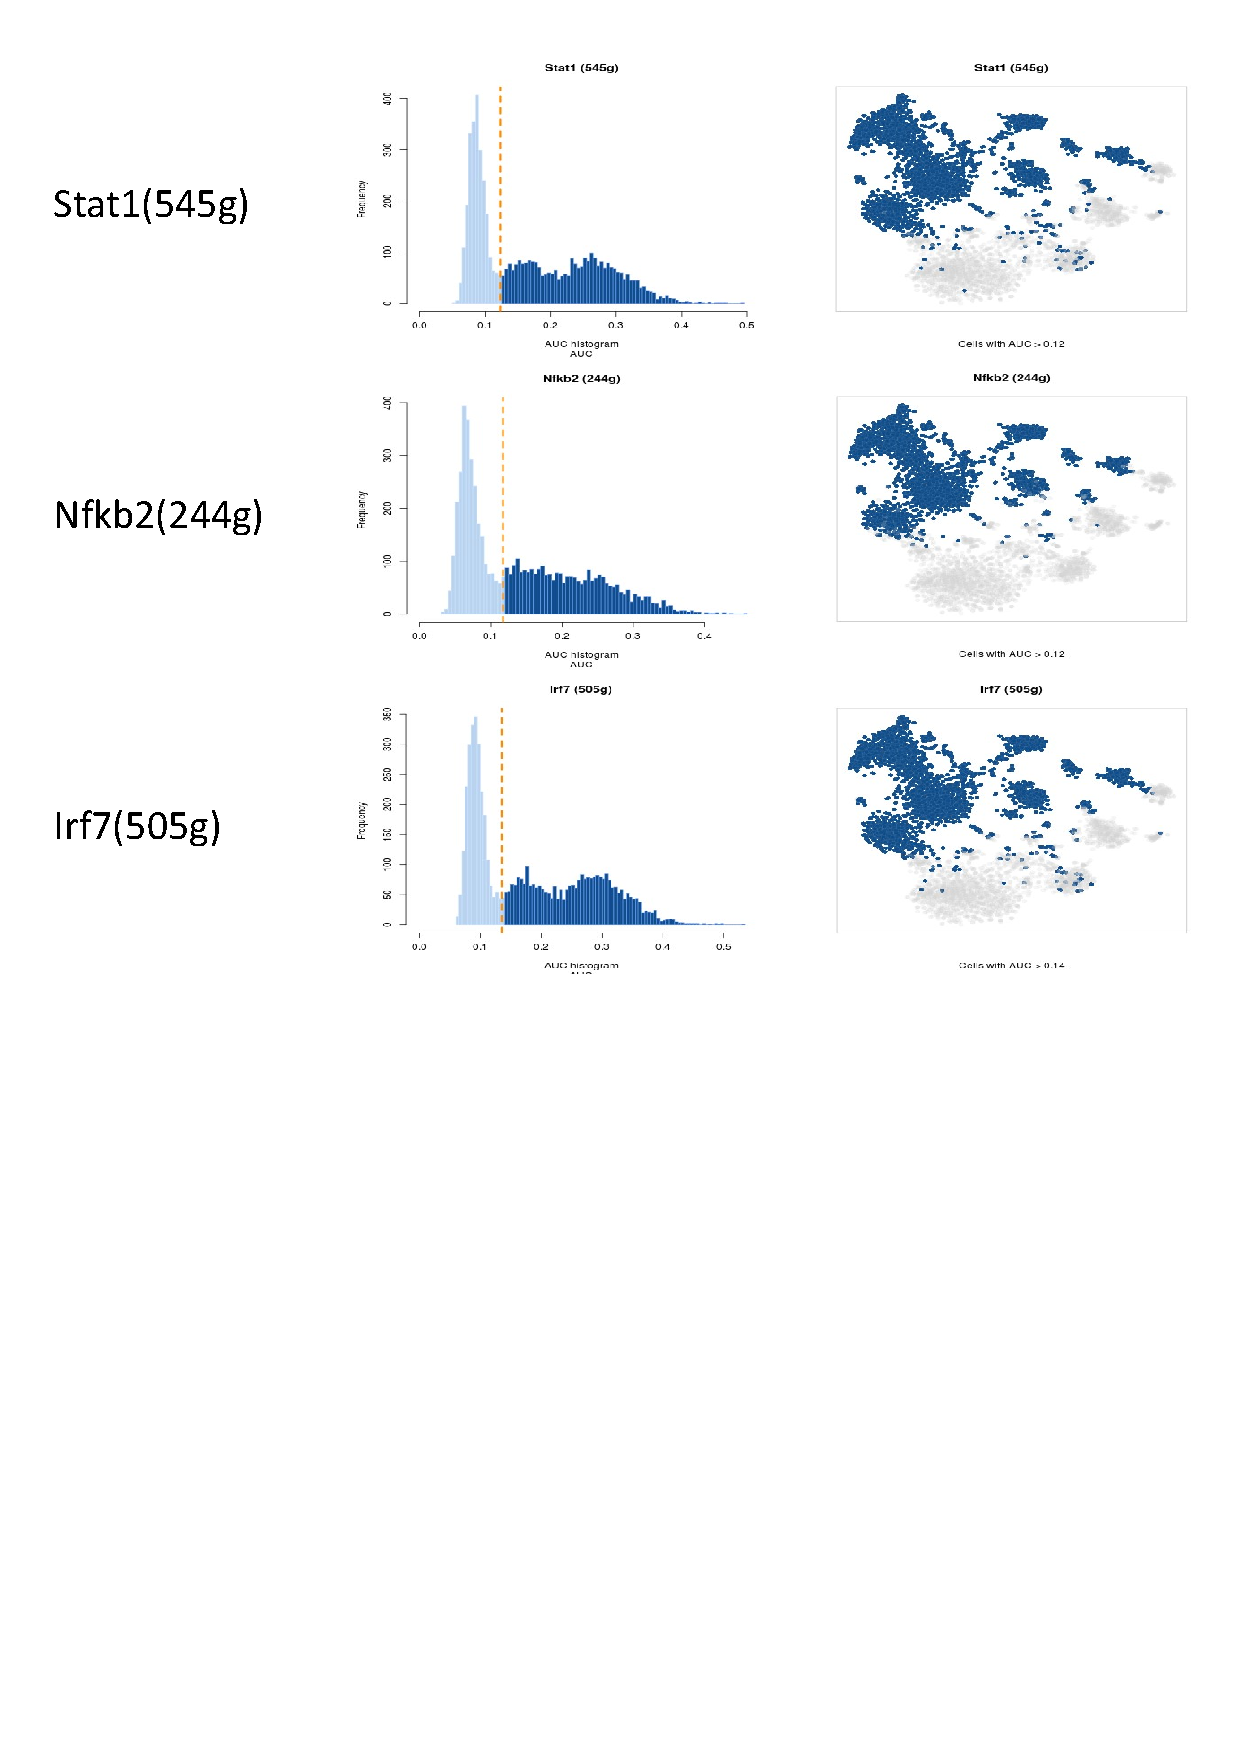
\includegraphics[width=0.8\textwidth]{figs/expr-fig3.pdf}
  \caption{具备双峰分布或者重尾分布的转录因子}
  \label{fig:expr-fig3}
\end{figure}

\section{讨论和未来工作}
  我们在实验中发现,在给以小鼠$TNF-\alpha$刺激之后,其部分垂体细胞在经历UMAP可视化降维之后,呈现出与其他炎症状态细胞相分离的现象。这似乎意味着垂体细胞在参与中枢神经内分泌炎症调节过程中,会因免疫刺激不同而进入不同的调节状态。

  我们初步推断是$TNF-\alpha$作为一种较强的免疫刺激剂,使垂体细胞进入一种不可逆转的免疫状态。在实验设计上,针对LPS、saline与Ploy I:C,我们都设计了长短恢复时程的对比试验,但$TNF-\alpha$只有短时程恢复处理。其原因在于$TNF-\alpha$相比LPS、Ploy I:C产生的免疫反应过于剧烈,小鼠在被腹腔注射500ug$TNF-\alpha$之后无法恢复,6h内便会死亡。

  我们未来的工作便打算在该研究的基础上,进一步探讨面对不可恢复炎症刺激与可恢复炎症刺激时垂体细胞在转录水平上的差异,揭示由健康(healthy)状态向这两种炎症(inflammation)状态转变的关键转录因子。

